
\documentclass{article} % For LaTeX2e
\usepackage[submission]{colm2025_conference}

\usepackage{microtype}
\usepackage{hyperref}
\usepackage{url}
\usepackage{booktabs}

\usepackage{lineno}

\definecolor{darkblue}{rgb}{0, 0, 0.5}
\hypersetup{colorlinks=true, citecolor=darkblue, linkcolor=darkblue, urlcolor=darkblue}

% Editors
\definecolor{maria-color}{HTML}{7881F2}
\newcommand{\maria}[1]{{\color{maria-color}[#1]$_{MA}$}}

% TODO's
\definecolor{todo-color}{HTML}{ff3232}
\newcommand{\todo}[1]{{\color{todo-color}[#1]}}
\newcommand\todocite{{\color{red}{CITE}}\xspace}

% Highlights colors.
\definecolor{lightblue}{RGB}{212, 235, 255}
\definecolor{orange}{RGB}{255, 105, 0}
\definecolor{lightgreen}{RGB}{177, 231, 171}
\definecolor{lightyellow}{RGB}{255, 255, 148}

% Tables
\usepackage{booktabs}
\usepackage{array}
% \newcolumntype{P}[1]{>{\centering\arraybackslash}p{#1}}
% \newcolumntype{L}[1]{>{\raggedright\let\newline\\\arraybackslash\hspace{0pt}}p{#1}}
% \newcolumntype{R}[1]{>{\raggedleft\arraybackslash}p{#1}}
% \newcommand\tworows[1]{\multirow{2}{*}{\shortstack[l]{#1}}}
% \newcommand\tworowsc[1]{\multirow{2}{*}{\shortstack[c]{#1}}}
% \newcommand\threerows[1]{\multirow{3}{*}{\shortstack[l]{#1}}}

% Links
\usepackage{hyperref}

% Figures
\usepackage{float}
\usepackage{subcaption}
\usepackage{graphicx}

\usepackage{fontawesome5}
\usepackage{fancyhdr}
% \usepackage{soul}

% Nice colors
\definecolor{1-color}{HTML}{e6d4fa}
\definecolor{2-color}{HTML}{cff5f5}
\definecolor{3-color}{HTML}{d4fae6}
\definecolor{4-color}{HTML}{f9d4fa}
\definecolor{5-color}{HTML}{fae6d4}

% \usepackage[sort, numbers]{natbib}
\usepackage{float}
\usepackage{enumitem}
\usepackage{tcolorbox}

% EMOJIS
% \usepackage{scalerel,xparse}
% \NewDocumentCommand\thought{}{
%     \includegraphics[scale=0.2]{resources/icons8-thought-bubble.pdf}
% }
% \NewDocumentCommand\speech{}{
%     \includegraphics[scale=0.2]{resources/icons8-sms.pdf}
% }

% BIBLIOGRAPHY
\usepackage{natbib}


\title{Extended Abstract: New Narrative Annotation Infrastructure in the Modern Social Media Ecosystem}

% Authors must not appear in the submitted version. They should be hidden
% as long as the \colmfinalcopy macro remains commented out below.
% Non-anonymous submissions will be rejected without review.

\author{Antiquus S.~Hippocampus, Natalia Cerebro \& Amelie P. Amygdale \thanks{ Use footnote for providing further information
about author (webpage, alternative address)---\emph{not} for acknowledging
funding agencies.  Funding acknowledgements go at the end of the paper.} \\
Department of Computer Science\\
Cranberry-Lemon University\\
Pittsburgh, PA 15213, USA \\
\texttt{\{hippo,brain,jen\}@cs.cranberry-lemon.edu} \\
\And
Ji Q. Ren \& Yevgeny LeNet \\
Department of Computational Neuroscience \\
University of the Witwatersrand \\
Joburg, South Africa \\
\texttt{\{robot,net\}@wits.ac.za} \\
\AND
Coauthor \\
Affiliation \\
Address \\
\texttt{email}
}

% The \author macro works with any number of authors. There are two commands
% used to separate the names and addresses of multiple authors: \And and \AND.
%
% Using \And between authors leaves it to \LaTeX{} to determine where to break
% the lines. Using \AND forces a linebreak at that point. So, if \LaTeX{}
% puts 3 of 4 authors names on the first line, and the last on the second
% line, try using \AND instead of \And before the third author name.

\newcommand{\fix}{\marginpar{FIX}}
\newcommand{\new}{\marginpar{NEW}}

\begin{document}

\ifcolmsubmission
\linenumbers
\fi

\maketitle

% \begin{abstract}
% We present a work-in-progress research plan for the construction of a new narrative annotation project on the social media platform Bluesky.
% Our high level goal is to address one of the major challenges facing online information ecosystems: the spread of narratives that support misinformation, conspiracy theories, and other misleading political content.
% We believe this problem needs the input of not only narrative researchers, but also experts in folklore, sensemaking, machine learning, and other disciplines, as well as the input by and collaboration with social media community members.
% To support this collaboration, we propose a flexible annotation tool which can be used to assign different kinds of narrative labels to social media posts, visible via personalized dashboards and re-usable by different research groups.
% \end{abstract}



\begin{figure}[h]
    \centering
    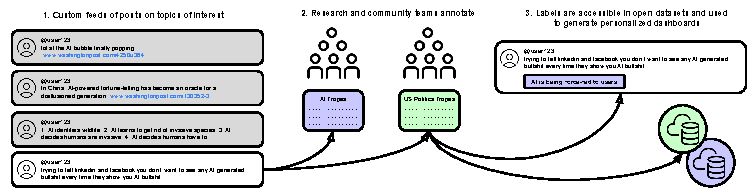
\includegraphics[width=\textwidth]{images/gnif_figure_bluesky.pdf}
     \caption{System overview of label contributors and their effect on the feed. Independent teams of annotators (including researchers, community members, and other volunteers) can flag posts for processing and then annotate posts using label sets of narrative tropes. Posts can be flagged anywhere on Bluesky and/or through a custom, topic-focused feed. These labels are then propagated to both personalized dashboards and to open datasets for other researchers to use and build upon.}
    \label{figure:system-overview}
\end{figure}


%%%%%%%%%%%%%%%%%%%%%%%%%%%%%%%%%%%%%%%%%%%%
% \section{Introduction}

% \begin{quote}
%     \textit{``I’ve been thinking about this a lot lately ... about how the frame of disinformation has failed us and what we can do differently. The problem is less about `units of facts,' right? The problem is with these big, sticky stories, and a lot of these stories are hundreds of years old.''} \\
%     -- Alice Marwick, director of research at Data \& Society; January, 2025
% \end{quote}

% The modern social media ecosystem is in crisis.
% While surveillance capitalism and tech monopolies have long controlled the most popular social media platforms, recent events have created a narrative stranglehold over most social media.
% Elon Musk's 2023 purchase of Twitter, now X, and his prioritizing and censoring of certain figures and content \citep{}, TikTok's internal censorship \citep{} as well as its threatened ban in the United States \citep{}, Facebook's reversion of its moderation rules \citep{}, the closure of Reddit, Facebook, X and other platforms to researchers \citep{}, newspaper conglomeration and purchase by tech billionaires \citep{}, and more have created an online information ecosystem where misinformation and disinformation can thrive unchecked.

The modern social media ecosystem is in crisis.
Recent events have created a stranglehold over most social media, with the purchase of Twitter by Elon Musk, TikTok's internal censorship and threatened U.S. ban, moderation changes at Meta, and the closing of research APIs supporting an online information ecosystem where misinformation and disinformation can thrive.
Attempts to check the spread of inaccurate content have not met with much success.
Technical challenges, such as the automatic detection of misinformation at scale, make tackling the problem difficult for engineers; expert fact checkers are not always trusted and have limited capacity to moderate entire social media platforms, let alone the whole of the internet; and crowdsourced projects like Community Notes (formerly Birdwatch), while promising, are gameable and limited in scope and speed \citep{wojcik2022birdwatchcrowdwisdombridging,allen2022birds,borenstein2025communitynotesreplaceprofessional}.

But more importantly, battling to correct individual pieces of misinformation is perhaps always a losing game, one that is simply not possible to win; not just because of the scale of the problem but because the larger persuasive goal of this misinformation might have nothing to do with the \textit{information} itself but instead its contribution to (1) a larger weakening of trust in all information and (2) the construction of shared, potentially harmful \textit{narratives} that are harder to pin down and combat.
In the words of Alice Marwick, director of the nonprofit research institute Data \& Society, ``\textit{The problem is less about `units of facts'... The problem is with these big, sticky stories}'' \citep{clarke2025nobody}.

Studying such stories, whose specifics might vary but whose shapes can spread quickly and stubbornly across communities, will need the combined expertise of researchers from many different disciplines.
However, there is little shared infrastructure to facilitate ongoing joint ownership and collaboration between all narrative stakeholders; narrative labels, such as media frames \citep{card2015media}, moral foundations \citep{graham2013moral}, and tropes \citep{DBLP:conf/emnlp/0001ABYBA24}, exist in separate frameworks far away from the journalists, community members, engineers, and other researchers who might be able to contribute to such labeling projects. 
We need large, shared experiments and resources that enable new collaborations.
% narrative, folklore (the circulation of culture across and within social networks), sensemaking (processes by which communities create shared knowledge), and machine learning (both natural language processing and computer vision, to address these problems at scale).
% For example, prior work in computational folkloristics has used network analysis and natural language processing methods to measure and analyze how conspiracy theory narratives spread online, within and across social media platforms \citep{}.
% However, the closing of social media platforms to researchers and the siloing of different narrative research threads --- both from one another and from the studied community members --- has made collaboration difficult.

In this extended abstract, we propose an ambitious research plan to begin to address some of these challenges.
This experiment will focus on a single social media platform --- Bluesky --- which uses an open protocol and supports researcher- and user-driven projects. 
We outline here a set of requirements and design plans to create a \textbf{collaborative narrative labeling pipeline} on Bluesky.
This pipeline will bring together users and researchers to label the kinds of ``big, sticky stories'' that spread online by collaboratively annotating Bluesky posts with narrative labels.



% \paragraph{What do we mean by ``narrative''?}

% Narratives have many definitions depending on the subject matter and disciplinary perspective. 
% \citet{piper-etal-2021-narrative} put forward a set of features --- including a narrator, mode of telling, audience, situation, etc. --- that together define the presence of \textit{narrativity}, which might be measured on a scale.
% In works such as \citet{antoniak-etal-2024-people}, narratives are more related to story telling and the narration of a specific sequence of events. 
% That is, they are a series of related events experienced or made by certain characters \cite{antoniak-etal-2024-people,shokri-etal-2024-safe}.
% % In this work, we focus instead on a meaning of narrative that is more closely related to stereotypical narrative patterns that spread and recur across many texts and authors.
% % the vulgar term as found/used commonly in the English language, which further includes 
% % These narratives have also been explained as unfalsifiable \citep{christensen2022searchingstructureunfalsifiableclaims} or unsupported claims, which is a claim with low or no check-worthiness that typically conform to a set of viewpoints a person holds in given debate topic \citep{christensen2023promptconditiongenerateclassification}. 
% In our initial annotation experiments, we have focused on \textit{tropes}~\citep{DBLP:journals/corr/abs-2011-00092,DBLP:conf/emnlp/0001ABYBA24}, which represent themes or motifs that are both recurrent and recognizable. 
% Tropes are closely related to frames, which describe the types of information that are chosen to be emphasized in a given narrative in order to ``promote a particular interpretation''~\citep{entman2007framing}.
% However, the infrastructure we build is agnostic to the definition of narrative used by the research teams. 
% Our goal is to provide a way to automatically organize information in such a way as to be useful for downstream applications and users, e.g., fact checkers and cultural analysts.

% Tropes, narrative frames...
% Tropes have been defined in -- and so --. Using the [tropes paper], we can define trope as a theme or motif which has the following properties: It is recurrent, i.e., appears
% frequently in the responses; and it is consistent, i.e.,
% the statements which represent the trope can be
% grounded in a single abstract concept. 


\paragraph{Narratives and the health of information ecosystems}

Addressing misinformation in online spaces has traditionally been carried out by human agencies accompanied by automated fact-checking and claim verification systems to determine the veracity of individual posts \cite{guo-etal-2022-survey,gupta-etal-2021-lesa,Warren2025Show}. 
% Beyond isolated social media posts, determining the biases propagated by the source entity is more complex to determine. 
% In terms of media organizations, researchers have evaluated the credibility of news sources via external attributions \cite{baly-etal-2018-predicting,10.14778/2777598.2777603}. 
% However, surveys have recently shown that 
% % despite the prevalence of both misinformed contents and fact-checking efforts, 
% risk aversion to misinformation varies across countries \cite{Hoes2024,Knuutila2022}.  
% \cite{doi:10.1177/14648849241303249,Hellman2024}
But another approach to misinformation in online communities has been to consider shared, high-level narratives as vectors, rather than specific statements whose veracity about specific people and events can be fact-checked.
The field of \textit{computational folkloristics} \citep{abello2012computational} has used this approach to study emerging conspiracy theories and their spread across the internet \citep{shahsavari2020conspiracy,tangherlini2020automated}. 
These studies detect ``underlying narrative frameworks'' and the connections between them \citep{shahsavari2020conspiracy}.
Similarly, \textit{sensemaking} research, which examines how people construct shared knowledge, has included studies of when this sensemaking process goes awry; in these cases, ``facts'' are not always the issue but rather rumors and conspiracy theories that spread higher level ``misinterpretations and mischaracterizations'' \citep{starbird2024facts}. 
% In this setting, \textit{frames} are understood as sets of socially constructed expectations and explanatory structures that help guide people's interpretive processes as they encounter evidence and decide which evidence to prioritize \citep{klein2007data,starbird2024facts}.
Having access to high quality frames and being able to apply frames appropriately could be the difference between experts and those more susceptible to misinformation; and disinformation can be seen as manipulation of the sensemaking (and frame application) process \citep{klein2007data,starbird2024facts}.

% These various research directions --- misinformation, folkloristics, sensemaking --- will all be necessary to tackle the tangled problem of narrative's role in online ecosystems.


% \paragraph{Examples from Prior Work: Folksonomies, Wisdom of the Crowd, Narrative Databases}

% While much research attention has gone to researcher-driven annotation --- including both researcher-annotated data and data annotated by crowdworkers paid for and instructed by researchers --- there also exist large projects in which online community members work together to label narrative elements and misinformation.
% For example, collaborative tagging systems, known as \textit{folksonomies} \citep{smith2007tagging,vanderwa2007folksonomy}, have thrived in online reading communities like Goodreads and LibraryThing, which describe narrative qualities of texts, assign genre categories, and more \citep{antoniak2021tags}.
% Another example is the crowdsourced project Community Notes, formerly known as Birdwatch, on Twitter/X, which recruits users to add ``notes'' to posts they deem to contain misleading information \citep{wojcik2022birdwatchcrowdwisdombridging}.
% In both examples, a large number of users are self-motivated to participate in annotating and organizing their own community.

% There are also existing initiatives directly related to narratives (in the storytelling sense) such as a citizen science project by \citet{piper-etal-2024-social} which successfully recruited almost 2k volunteers to provide over 70k annotations, or the \textsc{LitBank}\footnote{\url{https://github.com/dbamman/litbank}}repository of book annotations (e.g., entities, events) \citep{bamman-etal-2019-annotated,sims-etal-2019-literary,bamman-etal-2020-annotated}.
% And there are dataset-centered projects like ISEBEL (Intelligent Search Engine for Belief Legends),\footnote{\url{https://isebel.eu/}} which consolidates data from different folktale databases.
% These projects have all created valuable resources for the narrative research community, and we aim to build on these efforts by (1) taking lessons about community involvement, (2) sharing open resources that can be used by different research groups, and (3) focusing our work on online social media as a first direction, as there is a gap for open, collaborative resources for narrative research in this space.


% What motivates people to participate in these systems... and this motivation gives us reason to believe we can include community members in this project.




%%%%%%%%%%%%%%%%%%%%%%%%%%%%%%%%%%%%%%%%%%%%
% \section{Proposed Study Design}

\paragraph{Prototype design}

Bluesky\footnote{\url{https://bsky.app/}} is a new social media platform built using the AT Protocol,\footnote{\url{https://atproto.com/}} a decentralized protocol for large-scale social web applications. 
% Federation means that data is stored on host servers and is portable; in theory, any user may move all of their Bluesky data to other applications.
% While Bluesky itself is still under construction and much remains uncertain about this platform and the future of the protocol, 
Bluesky's popularity and its open and ``hackable'' structure make it ideal for computational social experiments, such as the one we propose here. 
% Users and designers can create their own custom feeds (algorithmically sorted and filtered posts that other users can subscribe to), custom lists and ``starter packs'' (thematic lists of users), and moderation via \textit{labels}.
Bluesky labels\footnote{\url{https://docs.bsky.app/docs/advanced-guides/moderation}} can be designed and applied by any user who chooses to run a \textit{moderation service}.
Other users may then subscribe to any of these services, which can then hide, warn, or simply display a label for relevant content; the labels are all opt-in.
% Users have already begun using these moderation services creatively.
% While many moderation services are designed to capture and hide undesirable content, there are also many moderation services that apply labels that are meant to be viewed by subscribing users.
For example, one such service adds labels to the profiles of U.S. politicians with the names of their largest corporate donors.
% \footnote{U.S. Government Officials: \url{https://bsky.app/profile/us-gov-funding.bsky.social}}. 
% Other services allow individual users to apply pronoun or zodiac sign labels to their own profiles and view such labels on the profiles of others who have subscribed to the service.\footnote{Zodiac Sign Labels: \url{https://bsky.app/profile/did:plc:cdbp64nijvsmhuhodbuoqcwi}}



% \subsection{Narrative Labels}

% We wish to begin with a set of labels that are general enough to be able to organize posts into common narratives and narrative elements, but not so broad as to be all-encompassing topics or which capture high-level aspects of language.
% %The narrative labels should be specific enough to encompass a general trope within a discussion topic but not so broad as to be a topic of its own or general argumentation style.
% % For example a useful narrative label could identify content which exemplifies ``the generational gap'', which is a general theme/rhetorical device used in various debates and can be used to argue for a particular position. On the contrary, a topic such as ``quality of life'' is too broad to be considered a theme or motif and is additionally not an argumentation technique such as ``projection'' which accuses an opponent of underhanded tactics instead of arguing for a cause.
% Ideally, we will derive a flexible ontology such that our system will be able to handle multiple label sets which users and researchers can choose between, depending on their preferences and goals.
% We have two broad options of how to decide on a set of narrative labels.
% \begin{enumerate}
%     \item We can select a list of narrative labels from the known literature. 
%     \item We can design and curate a list of narrative labels ourselves, using our domain expertise and close reading and/or a model to generate these automatically. \textbf{We will begin with this option.}
% \end{enumerate}

% A variety of narrative labels have been defined in prior work which each capture different and potentially complementary aspects of narratives. 
% Here we describe \textit{frames}, \textit{moral sentiment}, and \textit{tropes}, which describe both meta-information about narratives (i.e., \textit{how} a narrative is presented) as well as help to organize narratives into common themes. 

% \paragraph{Media Frames} Frames are conceptual tools that both communicators and audiences use to interpret and categorize issues and events \cite{gidin1980whole} \cite{reese2001prologue}. By highlighting specific elements of a topic and minimizing others,communicators frame messages in ways they believe will resonate with audiences \cite{goffman1974frame} and can shape the way the topic is perceived by readers or viewers.  The motivation for framing analysis is that a piece of information or a narrative can be presented in many different ways, and framing provides a way of organizing information by which aspects of the information are emphasized. One of the most popular labeling schemes comes from the media frames corpus (MFC)~\cite{card2015media}, which consists of hand annotated news articles with fine-grained span level labels indicating the framing of those spans. The schema uses 15 different frames as defined in previous work~\cite{boydstun2014tracking}, consisting of labels such as \textit{Economic}, \textit{Morality}, and \textit{Health and Safety} frames, and has been used across multiple studies and multiple languages (e.g., for analyzing Russian media frames~\cite{DBLP:conf/emnlp/FieldKWPJT18} and for multi-modal framing analysis \cite{arora2025frame}).

% \paragraph{Character Frames} Similar to media frames, character frames seek to characterize how the entities or actors in a given narrative are presented. This is useful for organizing different narratives by their attitudes towards the entities that they describe. Within NLP, a schema which has been used in multiple studies~\cite{DBLP:conf/eacl/SharmaKSMNAC23,DBLP:journals/corr/abs-2205-07557} uses \textit{hero}, \textit{villain}, and \textit{victim} labels to identify the actors in narratives. 


%Heroes, Villains, and Victims \cite{sharma-etal-2023-characterizing}, and GPT-3: Automated Extraction of Character Roles Without Training Data (Dominik Stammbach, Maria Antoniak, Elliott Ash)

%The Media Frames Corpus: Annotations of Frames Across Issues (Dallas Card, Amber E. Boydstun, Justin H. Gross, Philip Resnik, Noah A. Smith)

%Framing and Agenda-setting in Russian News: a Computational Analysis of Intricate Political Strategies (Anjalie Field, Doron Kliger, Shuly Wintner, Jennifer Pan, Dan Jurafsky, Yulia Tsvetkov)

% \paragraph{Moral Sentiment} \textit{Moral sentiment} organizes information based on a combination of both moral category and polarity within that moral category. Works on automatically detecting the moral sentiment of text have focused on labels derived from Moral Foundations Theory~\cite{graham2013moral}, which proposes an ontology of human morality consisting of 5 moral categories and 2 labels for each category representing the polarity. These include care/harm, fairness/cheating, loyalty/betraying, authority/subversion, and purity/degradation. This taxonomy has been used as the base for multiple datasets in NLP across different domains, including Twitter/X~\cite{hoover2020moral} and Reddit~\cite{trager2022moral}.

% \paragraph{Tropes} 
% \textit{Tropes} organize information according to the common themes/motifs which the information embodies. A salient lexicon of tropes which has been used in the NLP community comes from TV Tropes,\footnote{TV Tropes \url{https://tvtropes.org}} a community-driven effort to catalogue the common themes and motifs expressed in different media. Examples of labels include themes such as ``The Hero's Journey'' and the ``Rags to Riches'' story. 
% An analysis of these tropes identifying gender bias was performed in~\cite{DBLP:journals/corr/abs-2011-00092}, demonstrating how tropes can reveal different biases across different media.
% \textbf{We will focus on topic-specific tropes in our first experiments.
% }
%Analyzing Gender Bias within Narrative Tropes (Dhruvil Gala, Mohammad Omar Khursheed, Hannah Lerner, Brendan O’Connor, Mohit Iyyer)

% In addition to existing labels, we could also curate or generate new narrative labels based on rounds of human curation and automatic analysis.
% Human curation would include teams of annotators who work independently to assign free-text themes to texts and then discuss until converging on a final, closed set of labels.
% This process could be supplemented by clustering or topic modeling of the data as well as LLM-generated labels.
% In initial experiments, we have used Claude 3.5 Sonnet to generate small sets of narrative labels.

% \todo{say more here, add some citations for how we might technically go about this generation process}


% \subsection{Data}

% Members of the research team will have three options for selecting data to label.
% They can label data live on their personal feeds, as they notice posts that are relevant to the trope label set.
% Alternatively, they can read through a custom feed of all Bluesky posts containing content related to the selected trope topic.
% We created this feed using Graze.social, and it contains a chronologically sorted list of all original posts and replies containing keywords and hashtags related to the chosen topic.
% Finally, the research team can also search using their own keywords or create their own custom feeds.


% \subsection{System Description}

Our working prototype uses the open-source Ozone\footnote{\url{https://github.com/bluesky-social/ozone}} library, built on top of skyware and ATProto, to provide a usable interface.
Figure \ref{figure:system-overview} shows an overview of our pipeline:
\begin{enumerate}
    \item Researchers, community members, journalists and others can propose their own topic-specific trope annotation tasks through a formal process. Once approved, these will form annotation teams.
    \item Annotators (researchers, community members, general users) who subscribe to the moderation service can flag posts and provide free text rationales and labels.
    \item Flagged posts enter a moderation queue for trusted members of the annotation team, who can iteratively cluster and assign labels.
    \item Assigned labels and the associated Bluesky post IDs will be immediately available to researchers, builders, and general users via downloadable datasets and personalized dashboards. Data will need to be ``re-hydrated'' each time it is used, to preserve users' agency to edit and delete their data.
\end{enumerate}

% This entire process will always be public and available to the research and user community.


In designing this pipeline, we envision an open infrastructure that will allow for collaboration across narrative research groups and a sharing of annotation resources.
All work will be done openly, with both resources and results shared with the community.
This project will also include social media users, inviting them into the annotation process and allowing them to own their annotations and data while also sharing with researchers and other users and builders.
While the scope of this project is ambitious, it is urgent that more open, transparent, and centralized tools are designed for the new social media ecosystem.





%%%%%%%%%%%%%%%%%%%%%%%%%%%%%%%%%%%%%%%%%%%%
% \section{Impacts}
% % \textcolor{blue}{We should add a point to make some connection/comparison with 1 community note and 2 with semi-moderated platforms like Reddit and distributed platforms like Mastodon. Like how scalable and replicable our system is under different setups.}

% The entire pipeline will always be public and available to the research and user community. We hope this project will achieve the following outcomes.

% \paragraph{Useful narrative annotations on a growing social medial platform}
% The labels we apply to Bluesky posts will support research on the spread of narratives, the correlation between particular narratives and different topics (e.g., politics and healthcare), and provide a way of organizing and observing the content on Bluesky with respect to how that content is presented which may be useful for content moderation. These narrative labels will enable researchers to identify patterns in online discourse, as well as types of discourse which are helpful or harmful. In doing so, this will help perform content moderation by identifying posts and people which spread harmful and misinformative narratives.
% Apart from providing an alternative mechanism to examine the spread of misinformation, a byproduct of employing narrative labels would be to enable users to have better control over their recommendations/feeds in online spaces. Moreover, a better understanding of narratives can help in the development of games and training modules for media literacy \cite{Devasia2024,10.1093/pubmed/fdae050}.

% \paragraph{A new approach to misinformation} 
% As described previously, the current online information ecosystem is rife with misinformation, and the existing guardrails to prevent it are deteriorating. 
% Our study will provide a new way to combat harmful online content, including misinformation, which focuses on the ``big, sticky stories'' that are spread as opposed to the individual fact-checking. We and other research teams will provide sets of labels that encapsulate different aspects of narratives, and allow the research community to connect individual units of information into a coherent whole. 
% In doing so, our work goes beyond a narrow view of factuality, focusing on how to characterize online content more holistically, and involving the community of study and contributing back to that community through the creation of a live, customizable moderation service.
%\todo{write something here}


% \paragraph{Collaboration across narrative research groups}
% \todo{write something here}

% \paragraph{Collaboration with community members}
% \todo{write something here}




% %%%%%%%%%%%%%%%%%%%%%%%%%%%%%%%%%%%%%%%%%%%%
% \section{Limitations}

% \todo{just one platform for now, start with a limited label set and then scale up, ``narrative'' can mean many different things, any limitations about Bluesky that we want to highlight}




% %%%%%%%%%%%%%%%%%%%%%%%%%%%%%%%%%%%%%%%%%%%%
% \subsection{Ethical Considerations}

% We plan to follow a set of ethical guidelines informed by prior work and the specific affordances of Bluesky.
% First, because online narratives can involve sensitive, personal, or context-specific user-generated content, the protection of user privacy in such cases should involve not sharing raw user data or identifiable information, despite the original data being posted publicly.
% Practically, this means that we will anonymize or paraphrase the content when sharing examples in publications in order not to disclose specific user contributions, yet still be able to maintain the integrity of the narratives. 
% We will also not share data that includes raw posts created by users and instead share URLs or IDs that link back to those posts; this preserves users' agency over their content, so that they can edit or delete and these changes will be reflected in new analyses.

% Openness and transparency are core goals of this research plan. 
% Openness of the work will allow other researchers and practitioners to understand, critique, and extend the results in a manner that strictly upholds data governance practices. 
% Because our system works on Bluesky, the labeling process will be done publicly and in the open. 
% Anyone can examine our moderation service and view the labels we are applying, the custom feeds we create for annotation, and the content and users contained in that feed.
% Tthe posts we will be labeling are created by users who can easily discover the labels we are applying to their posts, and this means that our research team will be held to a higher standard.
% Data annotation usually happens not secretly but quietly, far removed and not publicized to the users being labeled. 
% \textbf{By using Bluesky, we open up that annotation process to the user community}; they can observe, contest, critique, contribute to, or remove themselves from annotation.
% We hope that this will create a high trust environment for collaborations between different research groups, online communities, and designers and engineers.


\bibliography{BIB}
\bibliographystyle{colm2025_conference}

\end{document}
